  \let\negmedspace\undefined
\let\negthickspace\undefined
\documentclass[journal]{IEEEtran}
\usepackage[a5paper, margin=10mm, onecolumn]{geometry}
\usepackage{lmodern} % Ensure lmodern is loaded for pdflatex
\usepackage{tfrupee} % Include tfrupee package

\setlength{\headheight}{1cm} % Set the height of the header box
\setlength{\headsep}{0mm}     % Set the distance between the header box and the top of the text

\usepackage{gvv-book}
\usepackage{gvv}
\usepackage{cite}
\usepackage{amsmath,amssymb,amsfonts,amsthm}
\usepackage{algorithmic}
\usepackage{graphicx}
\usepackage{textcomp}
\usepackage{xcolor}
\usepackage{txfonts}
\usepackage{listings}
\usepackage{enumitem}
\usepackage{mathtools}
\usepackage{gensymb}
\usepackage{comment}
\usepackage[breaklinks=true]{hyperref}
\usepackage{tkz-euclide} 
\usepackage{listings}                                      
\def\inputGnumericTable{}                                 
\usepackage[latin1]{inputenc}                                
\usepackage{color}                                            
\usepackage{array}                                            
\usepackage{longtable}
\usepackage{multicol}
\usepackage{calc}                                             
\usepackage{multirow}                                         
\usepackage{hhline}                                           
\usepackage{ifthen}                                           
\usepackage{lscape}
\begin{document}
	
	\bibliographystyle{IEEEtran}
	\vspace{3cm}
	
	\title{6.5.18}
	\author{EE24BTECH11059 - Y Siddhanth}
	% \maketitle
	% \newpage
	% \bigskip
	{\let\newpage\relax\maketitle}
	
	\renewcommand{\thefigure}{\theenumi}
	\renewcommand{\thetable}{\theenumi}
	\setlength{\intextsep}{10pt} % Space between text and floats
	
	
	\numberwithin{equation}{enumi}
	\numberwithin{figure}{enumi}
	\renewcommand{\thetable}{\theenumi}
	
	
	\textbf{Question}:\newline
	A rectangular sheet of tin 45 cm by 24 cm is to be made into a box without top,
	by cutting off square from each corner and folding up the flaps. What should be
	the side of the square to be cut off so that the volume of the box is maximum ? \\
	\textbf{Solution: }\\
	To find the volume, we can see that the sides become $45-2x , 24-2x$ and the height after folding the sheet becomes $x$, thus volume can be written as:
	\begin{align}
		V(x) &= x(45-2x)(24-2x) \\ 
		&= 1080x - 138x^2 + 4x^3 \\		
		V^\prime(x) &= 1080 - 276x + 12x^2
	\end{align}
	Evaluating the constraints on $x$, 
	\begin{align}
		45 - 2x &> 0 \\ 24 - 2x&>0 \\ x &> 0\\
	\end{align}
	Thus, $0<x<12$. Checking the convexity of the function $V(x)$ under the constraints,
	\begin{align}
		V^{\prime\prime}(x) &= 24x - 276  \\ &= 12\brak{2x-23}
	\end{align}
	Clearly, $V(x)$ is convex when $x>11.5$. Due to varying convexity of the function under the constraints, the problem can't be expressed as a Convex Optimization Problem. \\
	Solving this problem with gradient ascent, 
	\begin{align}
		x_n &= x_{n-1} + \alpha V^\prime(x) \\
		&= x_{n-1} + \alpha\brak{1080 - 276 x_{n-1} + 12 x_{n-1}^2}
	\end{align}
	Choosing $x_0 = 1, \alpha = 0.01, \epsilon = 10^{-6}$, where it is said that $x_n$ has converged when $\abs{x_n - x_{n-1}} < \epsilon$, We get the the value of $x$ as,
	\begin{align}
		x &= 5 cm  \\ 
		V(x) &= 2450 \text{cm}^3
	\end{align}
	\begin{figure}[h!]
		\centering
		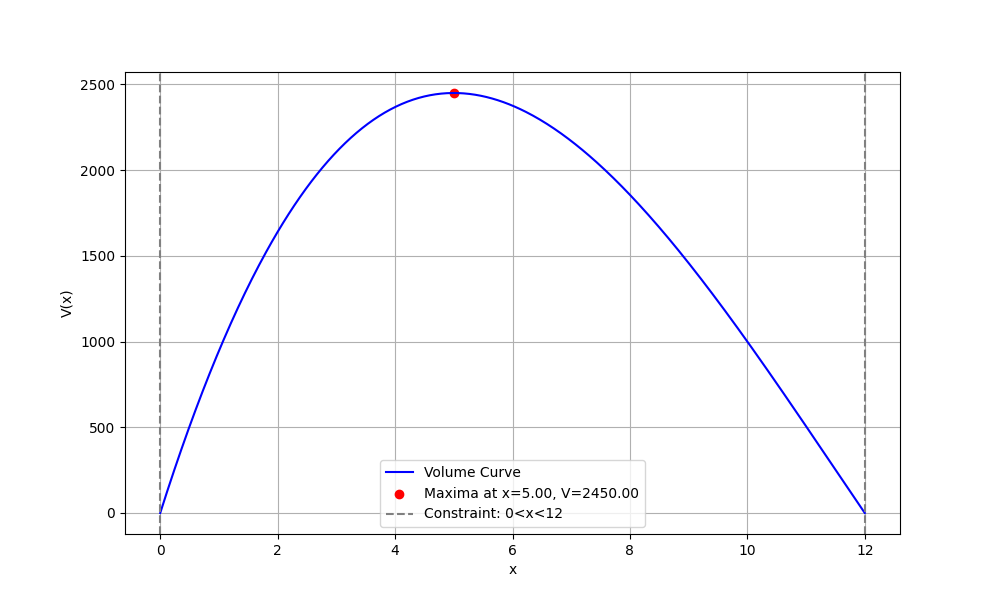
\includegraphics[width=\columnwidth]{figs/fig1.png}
		\caption{Maximum Value of the Volume Function}
		\label{stemplot}
	\end{figure}
	
\end{document}  